\documentclass[]{article}
\usepackage{lmodern}
\usepackage{amssymb,amsmath}
\usepackage{ifxetex,ifluatex}
\usepackage{fixltx2e} % provides \textsubscript
\ifnum 0\ifxetex 1\fi\ifluatex 1\fi=0 % if pdftex
  \usepackage[T1]{fontenc}
  \usepackage[utf8]{inputenc}
\else % if luatex or xelatex
  \ifxetex
    \usepackage{mathspec}
  \else
    \usepackage{fontspec}
  \fi
  \defaultfontfeatures{Ligatures=TeX,Scale=MatchLowercase}
\fi
% use upquote if available, for straight quotes in verbatim environments
\IfFileExists{upquote.sty}{\usepackage{upquote}}{}
% use microtype if available
\IfFileExists{microtype.sty}{%
\usepackage{microtype}
\UseMicrotypeSet[protrusion]{basicmath} % disable protrusion for tt fonts
}{}
\usepackage[margin=1in]{geometry}
\usepackage{hyperref}
\hypersetup{unicode=true,
            pdftitle={Generating Learning Curves},
            pdfauthor={Luis H. John, Xiaoyong Pan, Jenna Reps, Peter R. Rijnbeek},
            pdfborder={0 0 0},
            breaklinks=true}
\urlstyle{same}  % don't use monospace font for urls
\usepackage{color}
\usepackage{fancyvrb}
\newcommand{\VerbBar}{|}
\newcommand{\VERB}{\Verb[commandchars=\\\{\}]}
\DefineVerbatimEnvironment{Highlighting}{Verbatim}{commandchars=\\\{\}}
% Add ',fontsize=\small' for more characters per line
\usepackage{framed}
\definecolor{shadecolor}{RGB}{248,248,248}
\newenvironment{Shaded}{\begin{snugshade}}{\end{snugshade}}
\newcommand{\KeywordTok}[1]{\textcolor[rgb]{0.13,0.29,0.53}{\textbf{#1}}}
\newcommand{\DataTypeTok}[1]{\textcolor[rgb]{0.13,0.29,0.53}{#1}}
\newcommand{\DecValTok}[1]{\textcolor[rgb]{0.00,0.00,0.81}{#1}}
\newcommand{\BaseNTok}[1]{\textcolor[rgb]{0.00,0.00,0.81}{#1}}
\newcommand{\FloatTok}[1]{\textcolor[rgb]{0.00,0.00,0.81}{#1}}
\newcommand{\ConstantTok}[1]{\textcolor[rgb]{0.00,0.00,0.00}{#1}}
\newcommand{\CharTok}[1]{\textcolor[rgb]{0.31,0.60,0.02}{#1}}
\newcommand{\SpecialCharTok}[1]{\textcolor[rgb]{0.00,0.00,0.00}{#1}}
\newcommand{\StringTok}[1]{\textcolor[rgb]{0.31,0.60,0.02}{#1}}
\newcommand{\VerbatimStringTok}[1]{\textcolor[rgb]{0.31,0.60,0.02}{#1}}
\newcommand{\SpecialStringTok}[1]{\textcolor[rgb]{0.31,0.60,0.02}{#1}}
\newcommand{\ImportTok}[1]{#1}
\newcommand{\CommentTok}[1]{\textcolor[rgb]{0.56,0.35,0.01}{\textit{#1}}}
\newcommand{\DocumentationTok}[1]{\textcolor[rgb]{0.56,0.35,0.01}{\textbf{\textit{#1}}}}
\newcommand{\AnnotationTok}[1]{\textcolor[rgb]{0.56,0.35,0.01}{\textbf{\textit{#1}}}}
\newcommand{\CommentVarTok}[1]{\textcolor[rgb]{0.56,0.35,0.01}{\textbf{\textit{#1}}}}
\newcommand{\OtherTok}[1]{\textcolor[rgb]{0.56,0.35,0.01}{#1}}
\newcommand{\FunctionTok}[1]{\textcolor[rgb]{0.00,0.00,0.00}{#1}}
\newcommand{\VariableTok}[1]{\textcolor[rgb]{0.00,0.00,0.00}{#1}}
\newcommand{\ControlFlowTok}[1]{\textcolor[rgb]{0.13,0.29,0.53}{\textbf{#1}}}
\newcommand{\OperatorTok}[1]{\textcolor[rgb]{0.81,0.36,0.00}{\textbf{#1}}}
\newcommand{\BuiltInTok}[1]{#1}
\newcommand{\ExtensionTok}[1]{#1}
\newcommand{\PreprocessorTok}[1]{\textcolor[rgb]{0.56,0.35,0.01}{\textit{#1}}}
\newcommand{\AttributeTok}[1]{\textcolor[rgb]{0.77,0.63,0.00}{#1}}
\newcommand{\RegionMarkerTok}[1]{#1}
\newcommand{\InformationTok}[1]{\textcolor[rgb]{0.56,0.35,0.01}{\textbf{\textit{#1}}}}
\newcommand{\WarningTok}[1]{\textcolor[rgb]{0.56,0.35,0.01}{\textbf{\textit{#1}}}}
\newcommand{\AlertTok}[1]{\textcolor[rgb]{0.94,0.16,0.16}{#1}}
\newcommand{\ErrorTok}[1]{\textcolor[rgb]{0.64,0.00,0.00}{\textbf{#1}}}
\newcommand{\NormalTok}[1]{#1}
\usepackage{graphicx,grffile}
\makeatletter
\def\maxwidth{\ifdim\Gin@nat@width>\linewidth\linewidth\else\Gin@nat@width\fi}
\def\maxheight{\ifdim\Gin@nat@height>\textheight\textheight\else\Gin@nat@height\fi}
\makeatother
% Scale images if necessary, so that they will not overflow the page
% margins by default, and it is still possible to overwrite the defaults
% using explicit options in \includegraphics[width, height, ...]{}
\setkeys{Gin}{width=\maxwidth,height=\maxheight,keepaspectratio}
\IfFileExists{parskip.sty}{%
\usepackage{parskip}
}{% else
\setlength{\parindent}{0pt}
\setlength{\parskip}{6pt plus 2pt minus 1pt}
}
\setlength{\emergencystretch}{3em}  % prevent overfull lines
\providecommand{\tightlist}{%
  \setlength{\itemsep}{0pt}\setlength{\parskip}{0pt}}
\setcounter{secnumdepth}{5}
% Redefines (sub)paragraphs to behave more like sections
\ifx\paragraph\undefined\else
\let\oldparagraph\paragraph
\renewcommand{\paragraph}[1]{\oldparagraph{#1}\mbox{}}
\fi
\ifx\subparagraph\undefined\else
\let\oldsubparagraph\subparagraph
\renewcommand{\subparagraph}[1]{\oldsubparagraph{#1}\mbox{}}
\fi

%%% Use protect on footnotes to avoid problems with footnotes in titles
\let\rmarkdownfootnote\footnote%
\def\footnote{\protect\rmarkdownfootnote}

%%% Change title format to be more compact
\usepackage{titling}

% Create subtitle command for use in maketitle
\newcommand{\subtitle}[1]{
  \posttitle{
    \begin{center}\large#1\end{center}
    }
}

\setlength{\droptitle}{-2em}

  \title{Generating Learning Curves}
    \pretitle{\vspace{\droptitle}\centering\huge}
  \posttitle{\par}
    \author{Luis H. John, Xiaoyong Pan, Jenna Reps, Peter R. Rijnbeek}
    \preauthor{\centering\large\emph}
  \postauthor{\par}
      \predate{\centering\large\emph}
  \postdate{\par}
    \date{2018-09-23}

\usepackage{fancyhdr}
\pagestyle{fancy}
\fancyhead{}
\fancyhead[CO,CE]{Generating Learning Curves}
\fancyfoot[CO,CE]{PatientLevelPrediction Package Version 2.0.5}
\fancyfoot[LE,RO]{\thepage}
\renewcommand{\headrulewidth}{0.4pt}
\renewcommand{\footrulewidth}{0.4pt}

\begin{document}
\maketitle

{
\setcounter{tocdepth}{2}
\tableofcontents
}
\section{Introduction}\label{introduction}

This vignette describes how you can use the Observational Health Data
Sciences and Informatics (OHDSI)
\href{http://github.com/OHDSI/PatientLevelPrediction}{\texttt{PatientLevelPrediction}}
package to generate learning curves. This vignette assumes you have read
and are comfortable with building patient level prediction models as
described in the
\href{https://github.com/OHDSI/PatientLevelPrediction/blob/master/inst/doc/BuildingPredictiveModels.pdf}{\texttt{BuildingPredictiveModels}
vignette}.

Prediction models will show overly-optimistic performance when
predicting on the same data as used for training. Therefore,
best-practice is to partition our data into a training set and testing
set. We then train our prediction model on the training set portion and
asses its ability to generalize to unseen data by measuring its
performance on the testing set.

Learning curves assess the effect of training set size on model
performance by training a sequence of prediction models on successively
larger subsets of the training set. A learning curve plot can also help
in diagnosing a bias or variance problem as explained below.

\begin{figure}
\centering
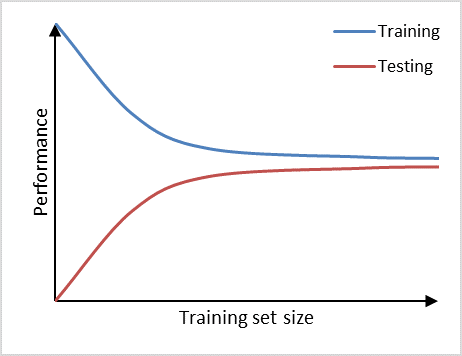
\includegraphics{learningCurve.png}
\caption{Learning curve example.}
\end{figure}

Figure 1, shows an example of learning curve plot in which the vertical
axis represents the model performance and the horizontal axis the
training set size. If training set size is small, the performance on the
training set is high, because a model can often be fitted well to a
limited number of training examples. At the same time, the performance
on the testing set will be poor, because the model trained on such a
limited number of training examples will not generalize well to unseen
data in the testing set. As the training set size increases, the
performance of the model on the training set will decrease. It becomes
more difficult for the model to find a good fit through all the training
examples. Also, the model will be trained on a more representative
portion of training examples, making it generalize better to unseen
data. This can be observed by the increasin testing set performance.

The learning curve can help us in diagnosing bias and variance problems
with our classifier which will provide guidance on how to further
improve our model. We can observe high variance (overfitting) in a
prediction model if it performs well on the training set, but poorly on
the testing set (Figure 2). Adding additional data is a common approach
to counteract high variance. From the learning curve it becomes
apparent, that adding additional data may improve performance on the
testing set a little further, as the learning curve has not yet
plateaued and, thus, the model is not saturated yet. Therefore, adding
more data will decrease the gap between training set and testing set,
which is the main indicator for a high variance problem.

\begin{figure}
\centering
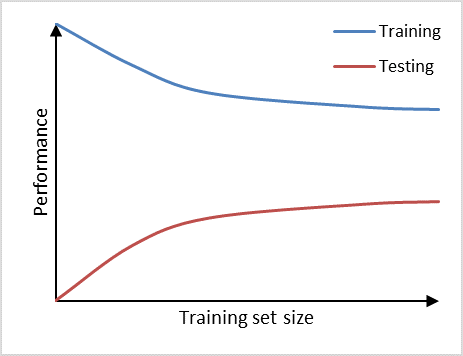
\includegraphics{learningCurveVariance.png}
\caption{Prediction model suffering from high variance.}
\end{figure}

Furthermore, we can observe high bias (underfitting) if a prediction
model performs poorly on the training set as well as on the testing set
(Figure 3). The learning curves of training set and testing set have
flattened on a low performance with only a small gap in between them.
Adding additional data will in this case have little to no impact on the
model performance. Choosing another prediction algorithm that can find
more complex (for example non-linear) relationships in the data may be
an alternative approach to consider in this high bias situation.

\begin{figure}
\centering
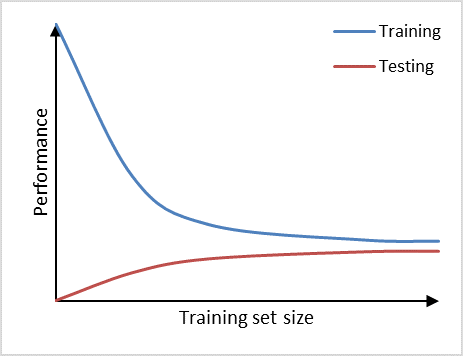
\includegraphics{learningCurveBias.png}
\caption{Prediction model suffering from high bias.}
\end{figure}

\section{Generating the learning
curve}\label{generating-the-learning-curve}

Use the
\href{http://github.com/OHDSI/PatientLevelPrediction}{\texttt{PatientLevelPrediction}}
package to generate a \texttt{population} and \texttt{plpData} object.
Alternatively, you can make use of the data simulator. The following
code snippet creates a population of 12000 patients.

\begin{Shaded}
\begin{Highlighting}[]
\KeywordTok{set.seed}\NormalTok{(}\DecValTok{1234}\NormalTok{)}
\KeywordTok{data}\NormalTok{(plpDataSimulationProfile)}
\NormalTok{sampleSize <-}\StringTok{ }\DecValTok{12000}
\NormalTok{plpData <-}\StringTok{ }\KeywordTok{simulatePlpData}\NormalTok{(}
\NormalTok{  plpDataSimulationProfile,}
  \DataTypeTok{n =}\NormalTok{ sampleSize}
\NormalTok{)}

\NormalTok{population <-}\StringTok{ }\KeywordTok{createStudyPopulation}\NormalTok{(}
\NormalTok{  plpData,}
  \DataTypeTok{outcomeId =} \DecValTok{2}\NormalTok{,}
  \DataTypeTok{binary =} \OtherTok{TRUE}\NormalTok{,}
  \DataTypeTok{firstExposureOnly =} \OtherTok{FALSE}\NormalTok{,}
  \DataTypeTok{washoutPeriod =} \DecValTok{0}\NormalTok{,}
  \DataTypeTok{removeSubjectsWithPriorOutcome =} \OtherTok{FALSE}\NormalTok{,}
  \DataTypeTok{priorOutcomeLookback =} \DecValTok{99999}\NormalTok{,}
  \DataTypeTok{requireTimeAtRisk =} \OtherTok{FALSE}\NormalTok{,}
  \DataTypeTok{minTimeAtRisk =} \DecValTok{0}\NormalTok{,}
  \DataTypeTok{riskWindowStart =} \DecValTok{0}\NormalTok{,}
  \DataTypeTok{addExposureDaysToStart =} \OtherTok{FALSE}\NormalTok{,}
  \DataTypeTok{riskWindowEnd =} \DecValTok{365}\NormalTok{,}
  \DataTypeTok{addExposureDaysToEnd =} \OtherTok{FALSE}\NormalTok{,}
  \DataTypeTok{verbosity =} \StringTok{"INFO"}
\NormalTok{)}
\end{Highlighting}
\end{Shaded}

Specify the prediction algorithm to be used.

\begin{Shaded}
\begin{Highlighting}[]
\CommentTok{# Use LASSO logistic regression}
\NormalTok{modelSettings <-}\StringTok{ }\KeywordTok{setLassoLogisticRegression}\NormalTok{()}
\end{Highlighting}
\end{Shaded}

Specify a test fraction and a sequence of training set fractions.

\begin{Shaded}
\begin{Highlighting}[]
\NormalTok{testFraction <-}\StringTok{ }\FloatTok{0.2}
\NormalTok{trainFractions <-}\StringTok{ }\KeywordTok{seq}\NormalTok{(}\FloatTok{0.1}\NormalTok{, }\FloatTok{0.8}\NormalTok{, }\FloatTok{0.1}\NormalTok{) }\CommentTok{# Create eight training set fractions}
\end{Highlighting}
\end{Shaded}

Specify the test split to be used.

\begin{Shaded}
\begin{Highlighting}[]
\CommentTok{# Use a split by person, alternatively a time split is possible}
\NormalTok{testSplit <-}\StringTok{ 'person'}
\end{Highlighting}
\end{Shaded}

Create the learning curve object.

\begin{Shaded}
\begin{Highlighting}[]
\NormalTok{learningCurve <-}\StringTok{ }\KeywordTok{createLearningCurve}\NormalTok{(population,}
                                     \DataTypeTok{plpData =}\NormalTok{ plpData,}
                                     \DataTypeTok{modelSettings =}\NormalTok{ modelSettings,}
                                     \DataTypeTok{testFraction =} \FloatTok{0.2}\NormalTok{,}
                                     \DataTypeTok{verbosity =} \StringTok{"TRACE"}\NormalTok{,}
                                     \DataTypeTok{trainFractions =}\NormalTok{ trainFractions,}
                                     \DataTypeTok{splitSeed =} \DecValTok{1000}\NormalTok{,}
                                     \DataTypeTok{saveModel =} \OtherTok{TRUE}\NormalTok{)}
\end{Highlighting}
\end{Shaded}

Plot the learning curve object (Figure 4). Specify one of the available
metrics: \texttt{AUROC}, \texttt{AUPRC}, \texttt{sBrier}.

\begin{Shaded}
\begin{Highlighting}[]
\KeywordTok{plotLearningCurve}\NormalTok{(}
\NormalTok{  learningCurve,}
  \DataTypeTok{metric=}\StringTok{'AUROC'}\NormalTok{,}
  \DataTypeTok{plotTitle =} \StringTok{'Learning Curve'}\NormalTok{,}
  \DataTypeTok{plotSubtitle =} \StringTok{'AUROC performance'}
\NormalTok{)}
\end{Highlighting}
\end{Shaded}

\begin{figure}
\centering
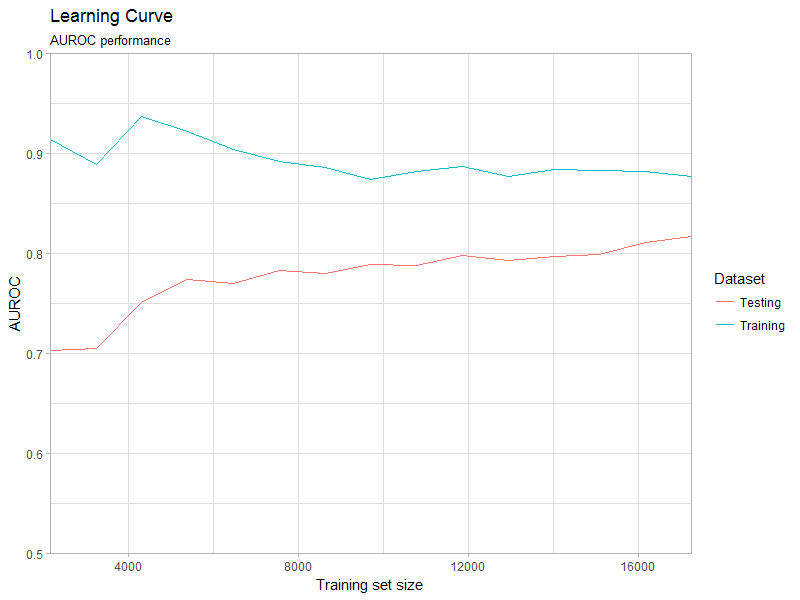
\includegraphics{learningCurvePlot.png}
\caption{Learning curve plot.}
\end{figure}

\section{Parallel processing}\label{parallel-processing}

The learning curve object can be created in parallel, which can reduce
computation time significantly. Currently this functionality is only
available for LASSO logistic regression. Depending on the number of
parallel workers it may require a significant amount of memory. We
advise to use the parallelized learning curve function for parameter
search and exploratory data analysis. Logging and saving functionality
is unavailable.

Use the parallelized version of the learning curve function to create
the learning curve object in parallel. R will find the number of
available processing cores automatically and register the required
parallel backend.

\begin{Shaded}
\begin{Highlighting}[]
\NormalTok{learningCurvePar <-}\StringTok{ }\KeywordTok{createLearningCurvePar}\NormalTok{(}
\NormalTok{  population,}
  \DataTypeTok{plpData =}\NormalTok{  plpData,}
  \DataTypeTok{modelSettings =}\NormalTok{ modelSettings,}
  \DataTypeTok{testSplit =}\NormalTok{ testSplit,}
  \DataTypeTok{testFraction =}\NormalTok{ testFraction,}
  \DataTypeTok{trainFractions =}\NormalTok{ trainFractions,}
  \DataTypeTok{splitSeed =} \DecValTok{1000}
\NormalTok{)}
\end{Highlighting}
\end{Shaded}

\section{Demo}\label{demo}

We have added a demo of the learningcurve to the Patient-Level
Prediction Package.

You can run the demos as follows:

\begin{Shaded}
\begin{Highlighting}[]
\CommentTok{# Show all demos in our package: }
 \KeywordTok{demo}\NormalTok{(}\DataTypeTok{package =} \StringTok{"PatientLevelPrediction"}\NormalTok{)}

\CommentTok{# Run the learning curve}
 \KeywordTok{demo}\NormalTok{(}\StringTok{"LearningCurveDemo"}\NormalTok{, }\DataTypeTok{package =} \StringTok{"PatientLevelPrediction"}\NormalTok{)}
\end{Highlighting}
\end{Shaded}

Do note that running this demo can take a considerable amount of time
(15 min on Quad core running in parallel)!

\section{Acknowledgments}\label{acknowledgments}

Considerable work has been dedicated to provide the
\texttt{PatientLevelPrediction} package.

\begin{Shaded}
\begin{Highlighting}[]
\KeywordTok{citation}\NormalTok{(}\StringTok{"PatientLevelPrediction"}\NormalTok{)}
\end{Highlighting}
\end{Shaded}

\begin{verbatim}
## 
##   Jenna Reps, Martijn J. Schuemie, Marc A. Suchard, Patrick B.
##   Ryan and Peter R. Rijnbeek (2018). PatientLevelPrediction:
##   Package for patient level prediction using data in the OMOP
##   Common Data Model. R package version 2.0.5.
## 
## A BibTeX entry for LaTeX users is
## 
##   @Manual{,
##     title = {PatientLevelPrediction: Package for patient level prediction using data in the OMOP Common Data
## Model},
##     author = {Jenna Reps and Martijn J. Schuemie and Marc A. Suchard and Patrick B. Ryan and Peter R. Rijnbeek},
##     year = {2018},
##     note = {R package version 2.0.5},
##   }
\end{verbatim}

\textbf{Please reference this paper if you use the PLP Package in your
work:}

\href{http://dx.doi.org/10.1093/jamia/ocy032}{Reps JM, Schuemie MJ,
Suchard MA, Ryan PB, Rijnbeek PR. Design and implementation of a
standardized framework to generate and evaluate patient-level prediction
models using observational healthcare data. J Am Med Inform Assoc.
2018;25(8):969-975.}


\end{document}
